\section{Robotic arm Kinematic Analysis}

\begin{frame}
\frametitle{Forward Kinematics}
\end{frame}

\begin{frame}
\frametitle{Inverse Kinematics - Decoupling Technique}
\end{frame}

\begin{frame}
\frametitle{Singularity points}
\end{frame}

\begin{frame}
\frametitle{RCM constraint}
\begin{center}
\begin{figure}[H]
\centering
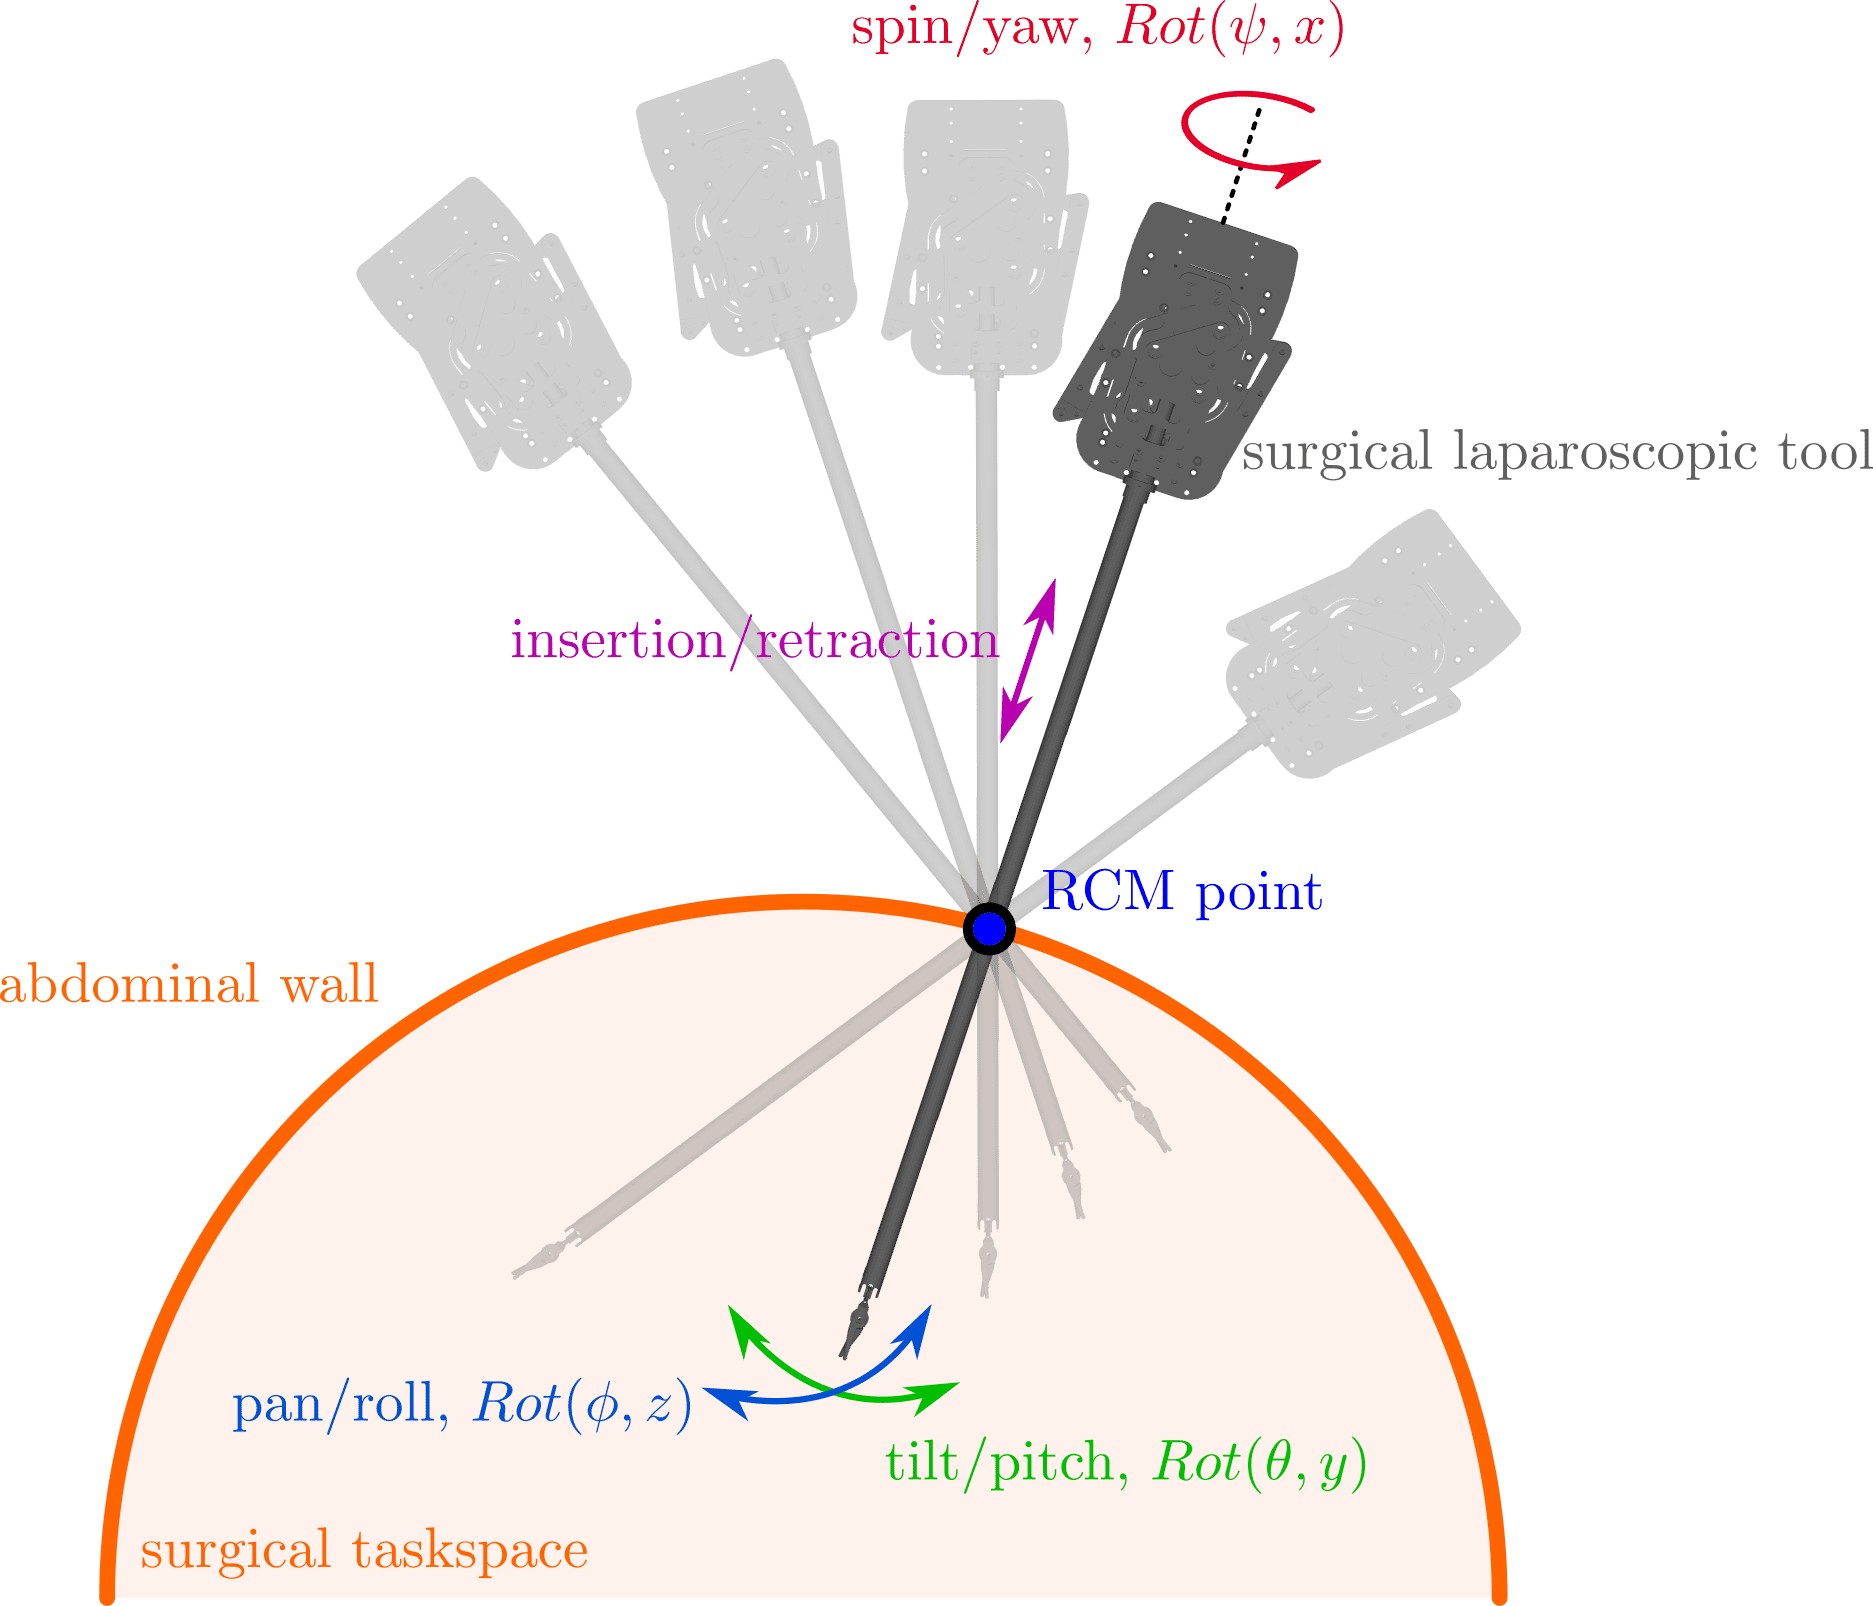
\includegraphics[width=0.5\textwidth]{../images/rcm-surgical-tool.png}\\
\caption{Illustration of pivoting motion of surgical laparoscopic tool around RCM point (also known as fulcrum or trocar point). Due to the RCM constraint, the tool has only 4 degrees of freedom.}
\end{figure}
\end{center}
\end{frame}

\begin{frame}
\frametitle{Elbow-up constraint}
\begin{columns}
\column{0.4\textwidth}
\begin{figure}[htbp]
\centering
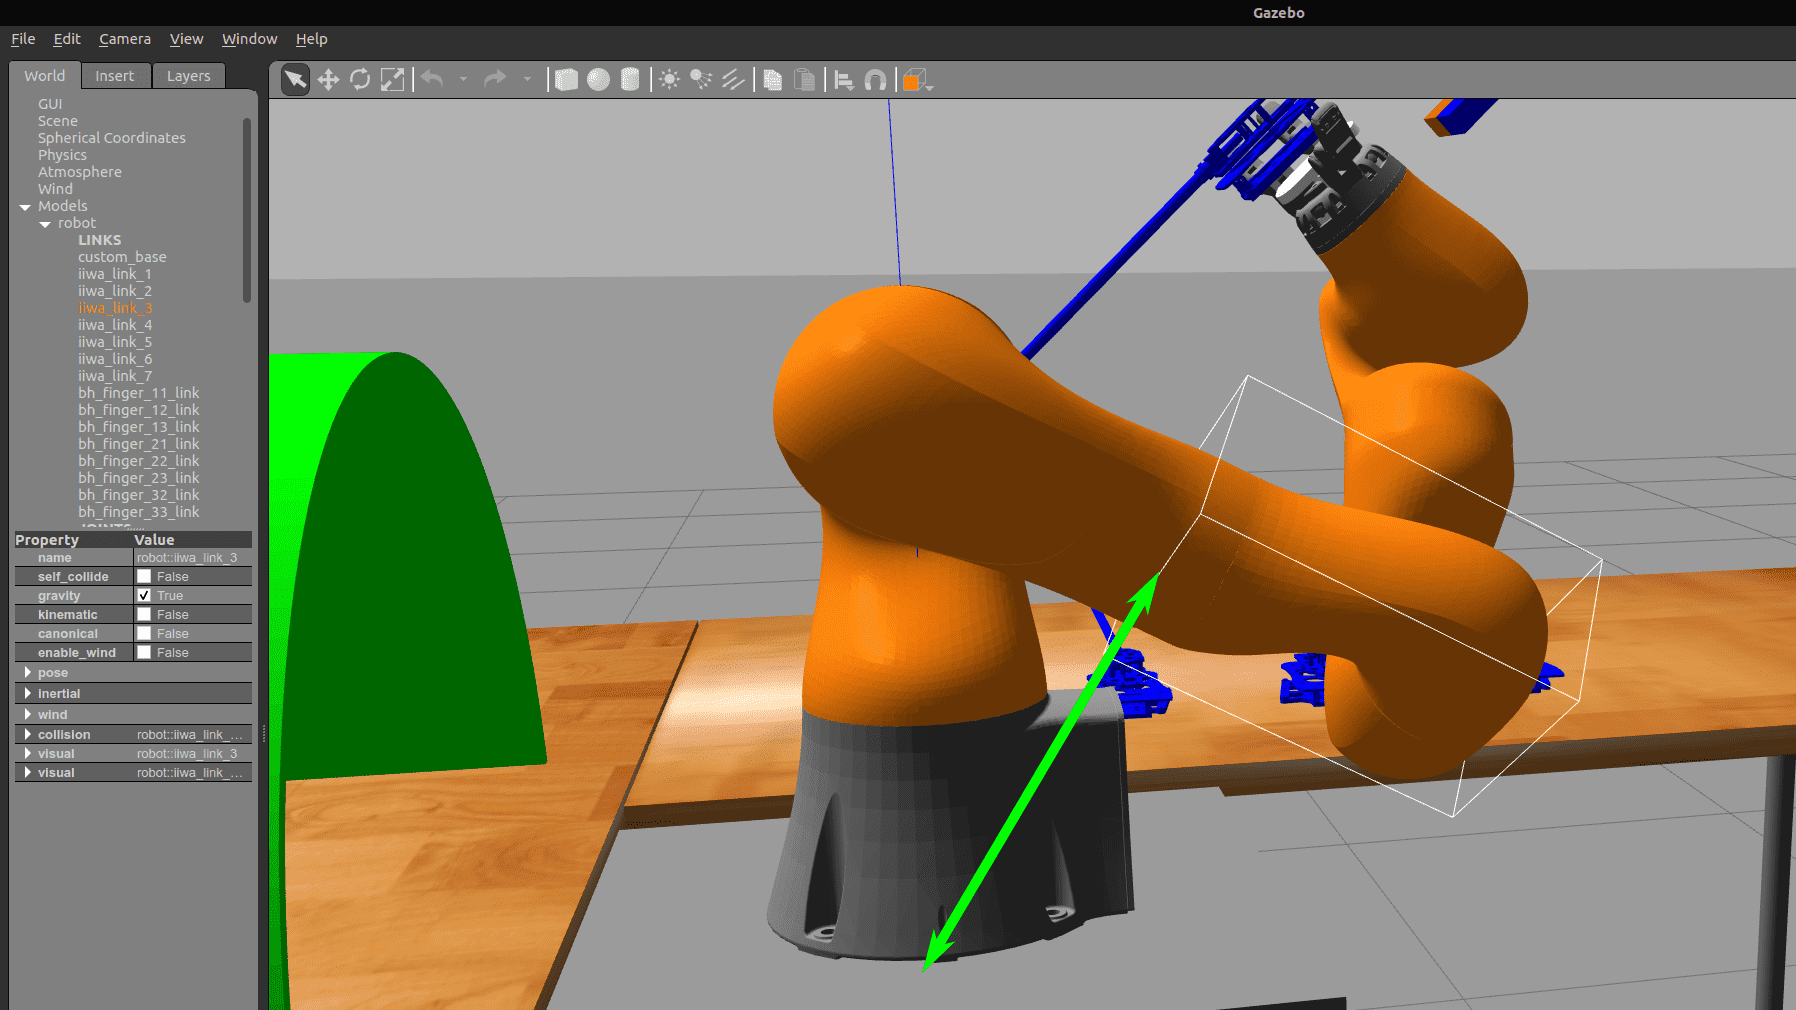
\includegraphics[width=\textwidth]{../images/elbow-down.png}\\
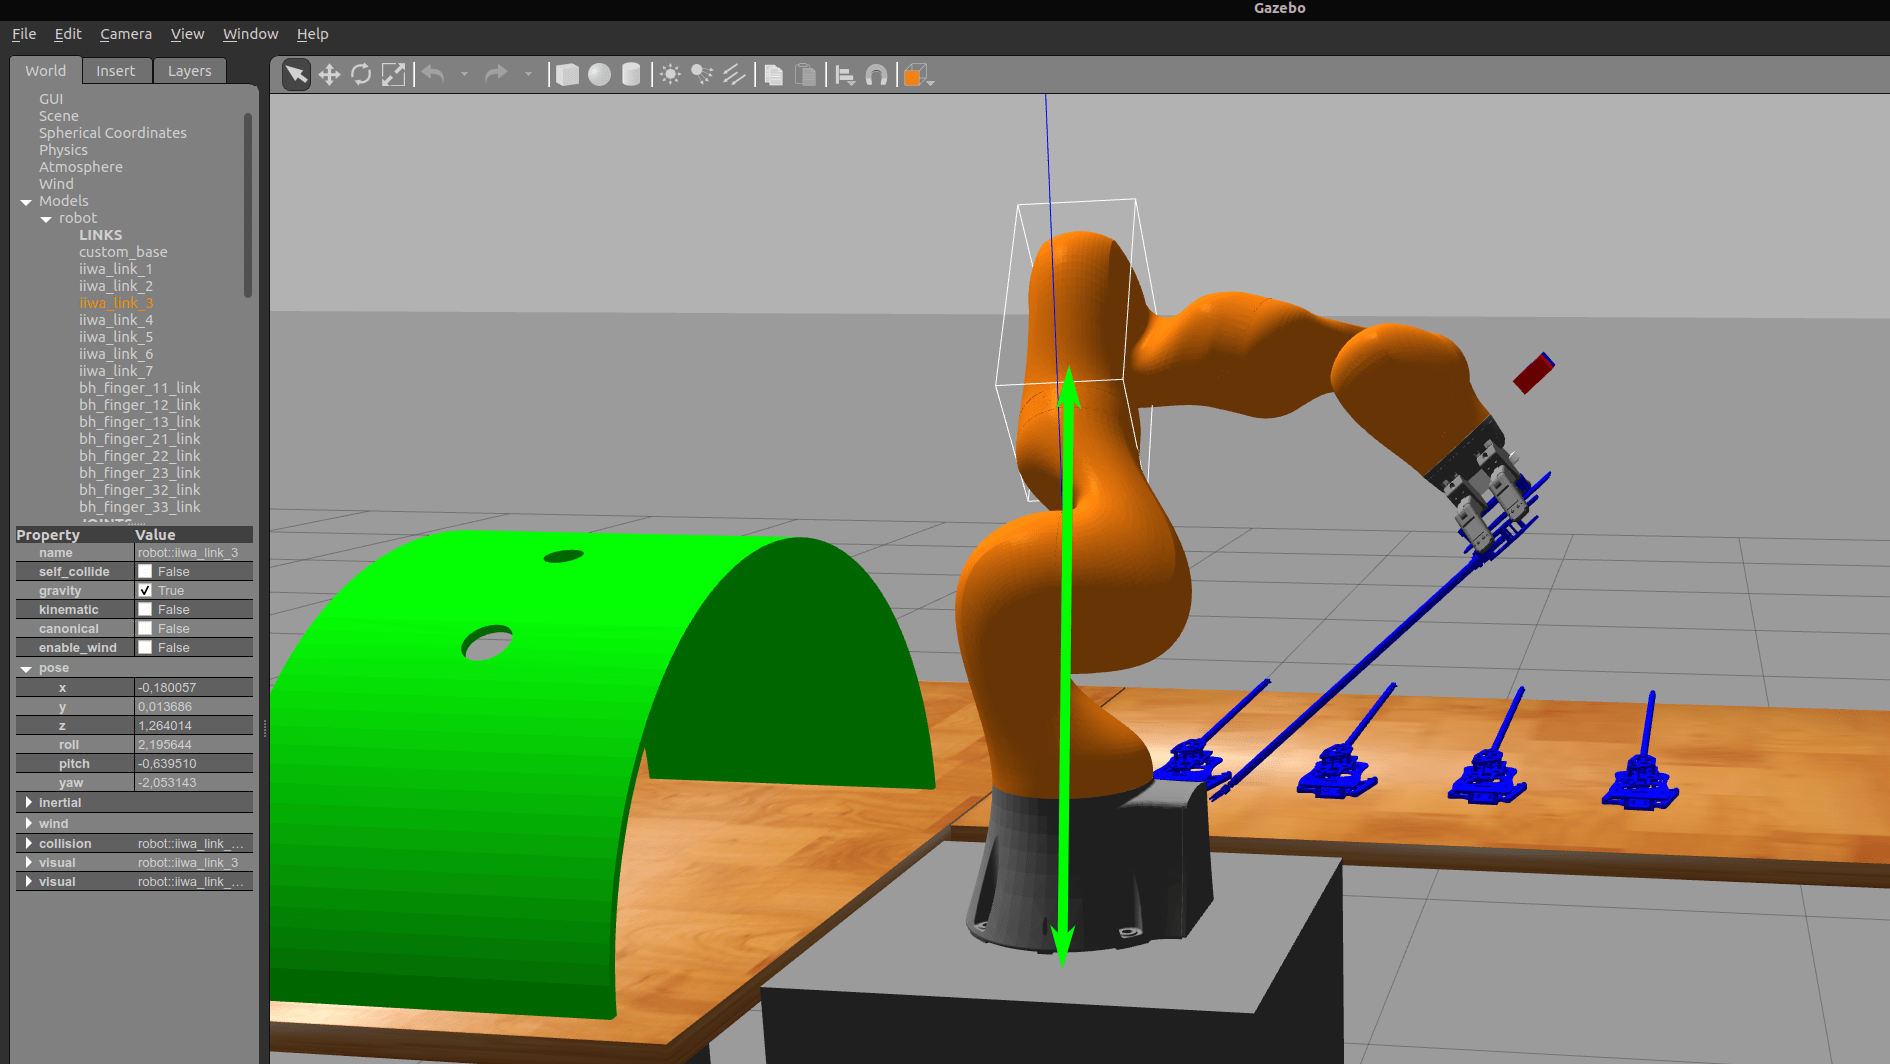
\includegraphics[width=\textwidth]{../images/elbow-up.png}\\
\caption{Top: elbow-down solution, bottom: elbow-up solution}
\label{elbow-up-vs-down}
\end{figure}

\column{0.6\textwidth}
\begin{figure}[htbp]
\centering
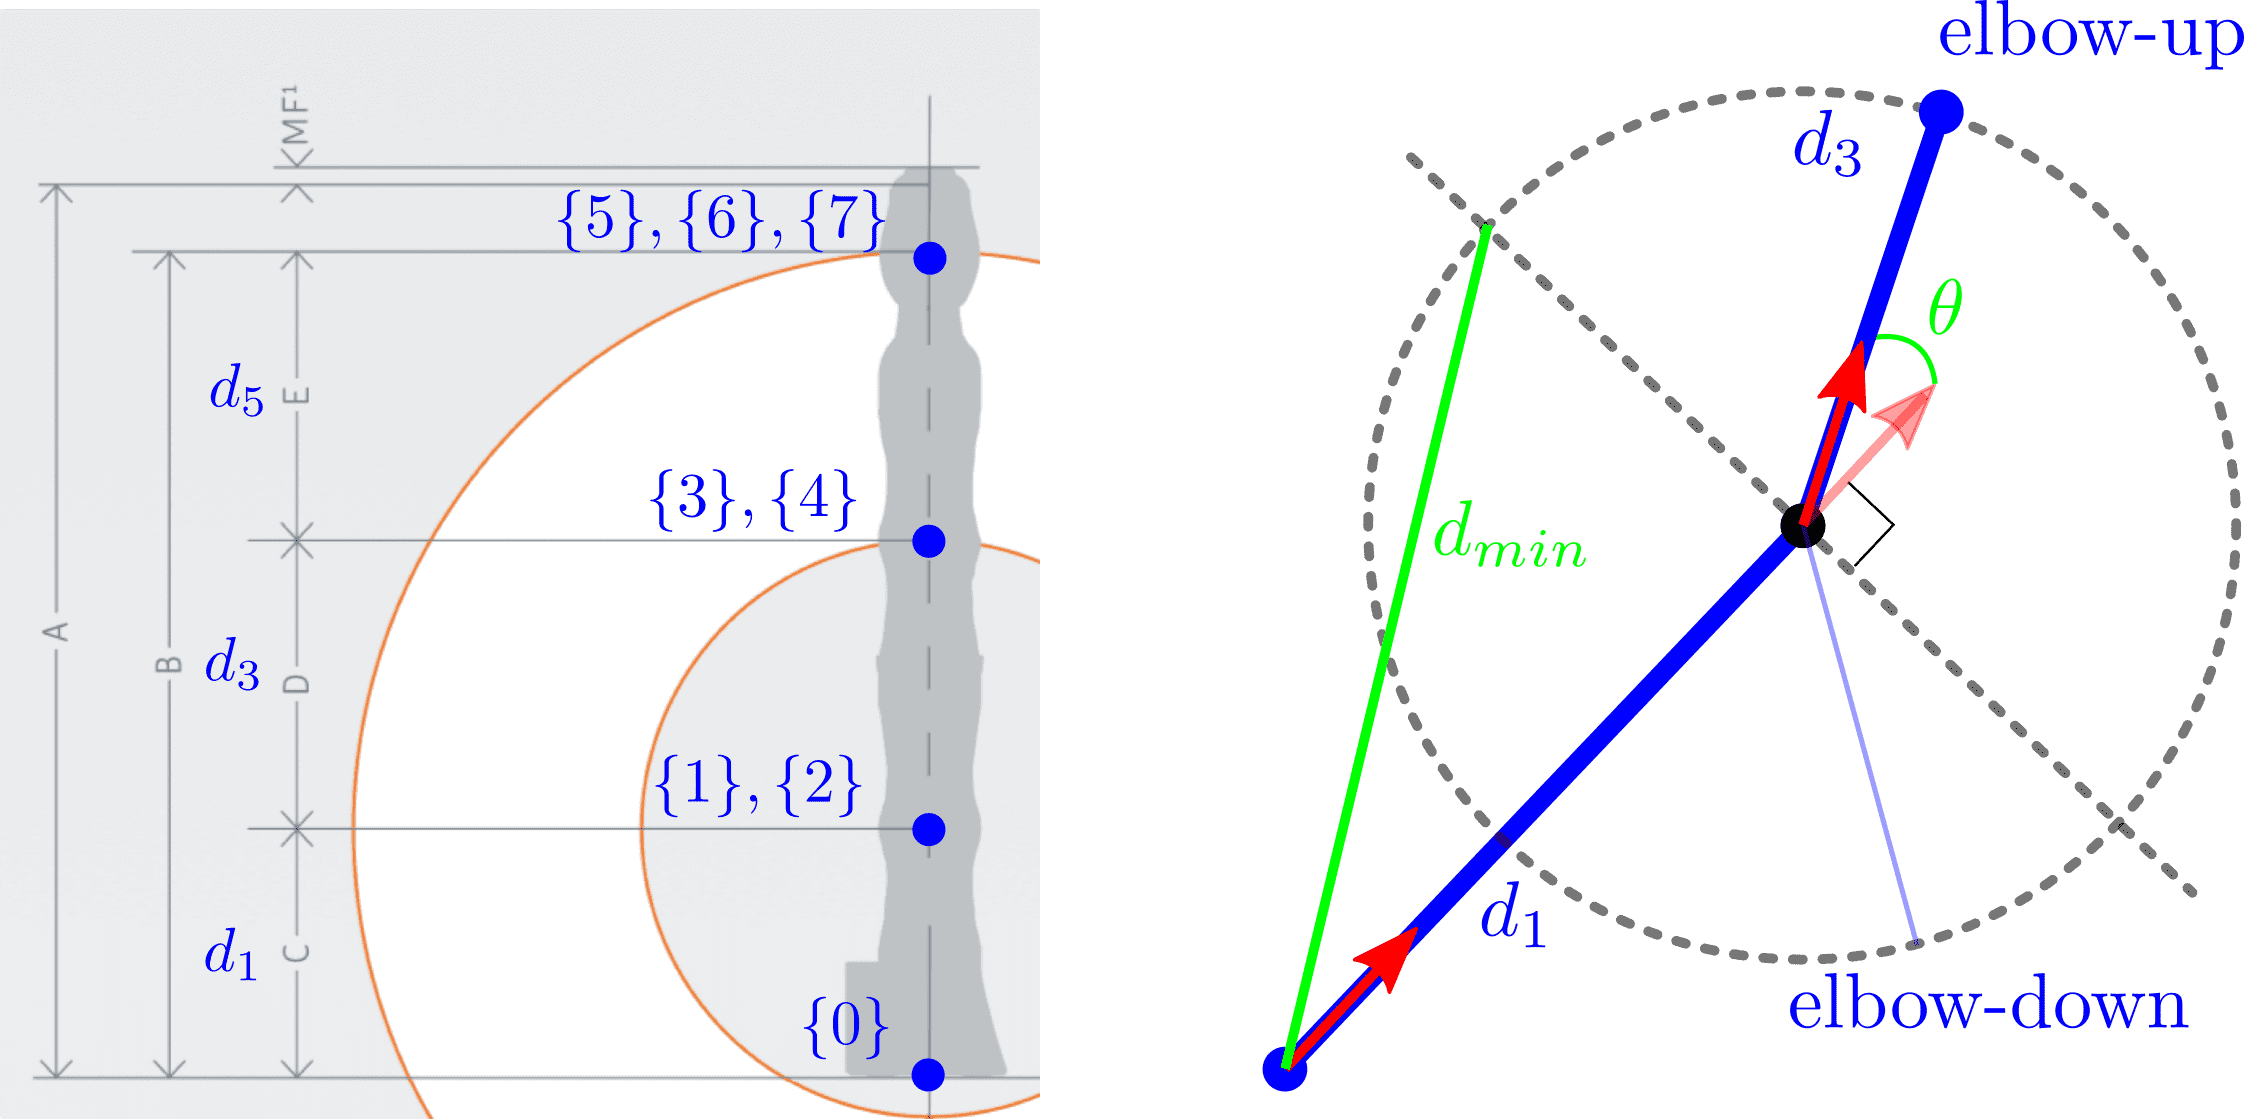
\includegraphics[width=0.8\textwidth]{../images/elbow-up-constraint-geometry.png}\\
\caption{Elbow-up constraint description with relative distance or angle between links with lengths $d_1$ and $d_3$}
\label{elbow-up-constraint-geometry}
\end{figure}

\begin{center}
$d_{\min} \leq d \leq d_{\max}$,
where
$d_{\min} = \sqrt{d_1^2 + d_3^2} = 553$mm and $d_{\max} = d_1 + d_3 = 780\mbox{mm}.$
\end{center}
\end{columns}
\end{frame}
